\documentclass{beamer}
% --------------- PACCHETTI ---------------
% Immagini
\usepackage{graphicx} 
% Layout multicolonna
\usepackage{multicol}
% Listings
\usepackage{listings}    
% ------------- FINE PACCHETTI ---------------


\usetheme{Copenhagen}

% --------------- INTESTAZIONE ---------------
\title{Verifica funzionale di programmi con Dafny}
\author{Lorenzo Quellerba}
\institute{Univeristà degli Studi di Torino}
\date{June 2023}
% --------------- FINE INTESTAZIONE ---------------

\begin{document}
\maketitle

% Il problema è definire come vogliamo dire le cose
% Dobbiamo parlare di:
% 1 - Introduzione a Dafny
% 2 - Minimo sindacale di teoria alla base
% 3 - Presentazione esempio albero

% Qua spieghi le caratteristiche del linguaggio:
% 1: Linguaggio oo con supporto anche funzionale (se lo vuoi dire)
% 2: Il processo di sviluppo in Dafny include anche la verifica funzionale 
% 3: Devi annotare programma con pre, post, inv, variant, e poi tutto a smt solver
% 4: Un programma Dafny poi può essere compilato in altri linguaggio di programmazione
\begin{frame}{Dafny}
    \begin{columns}[onlytextwidth]
        \column{0.7\textwidth}
        \begin{itemize}
            \item Dafny è un linguaggio di programmazione \textit{object oriented} che supporta sia il paradigma imperativo che quello funzionale
            \item Supporta la specifica formale attraverso precondizioni, postcondizioni, invarianti, varianti e i \textit{dynamic frames} per la formalizzazione delle modifiche della memoria
            \item La correttezza del codice viene verificata rispetto alla specifica data da un SMT solver (\textit{correct by construction})
            \item Al termine del processo di verifica un programma Dafny può essere compilato in altri linguaggi tra cui C++, Go, Java
        \end{itemize}
        \column{0.25\textwidth}
        \begin{figure}
            
\includegraphics[scale=0.4]{./assets/images/dafny-logo-230.png}
        \end{figure}
    \end{columns}
\end{frame}

\begin{frame}{Dafny: funzionamento}
    % Ora un veloce richiamo di teoria 
    % 1. Concetto alla base è quello di tripla di Hoare
    % 2. Per separare parte logica da parte sintattica usi wp calculus
    % 3. La formula che ottieni viene passata a SMT solver
    % 4. Grafico smt solver
    \only<1>{
    \begin{block}{Tripla di Hoare}
        \begin{center}
            \{P\}C\{Q\}     
        \end{center}
        Se l'asserzione \textit{P} è vera prima dell'esecuzione del comando \textit{C} allora l'asserzione \textit{Q} sarà vera al termine dell'esecuzione
    \end{block}
    \begin{block}{\textit{Predicate transformer semantics}}
        La semantica dei \textit{predicate transformer} è una riformulazione della logica di \textit{Floyd-Hoare} che definisce una strategia completa per la costruzione di deduzioni valide
    \end{block}
    \begin{block}{\textit{Weakest precondition}}
        Dato un comando \textit{C} e una postcondizione \textit{Q} la \textit{weakest precondition} (\textit{wp}) è un predicato \textit{$\phi$} tale per cui per ogni precondizione \textit{P}, \{P\}C\{Q\} se e solo se P$\implies \phi$
    \end{block}
    }
    \only<2>{
        \begin{figure}
            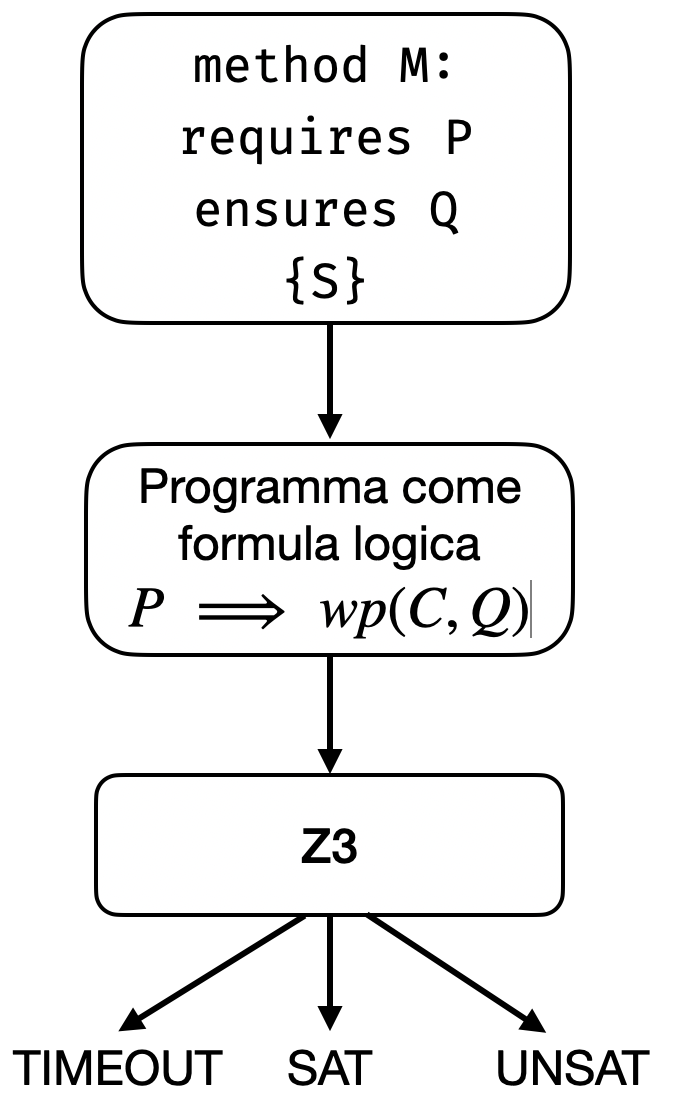
\includegraphics[scale=0.4]{./assets/images/mechanism.png}
        \end{figure}
    }
\end{frame}

\begin{frame}{Caratteristiche del linguaggio}
% Ora veramente in super sintesi le caratteristiche del linguaggio
% 1. Tipi
% 2. Generici
% 3. Predicati metodi e funzioni    
    \begin{itemize}
        \item Reference types e value types
        \item Generici
        \item predicati metodi funzioni classi
        \item 
    \end{itemize}
\end{frame}

\begin{frame}{Albero binario di ricerca}
% Albero binario di ricerca con veloce presentazione della struttura dati
    Richiamo di teoria della struttura
\end{frame}

\begin{frame}{BST: variabili d'istanza}
    \lstinputlisting[]{./assets/code/bst_instance_var.dfy}
\end{frame}

\begin{frame}{BST: invariante di struttura}
    \lstinputlisting[]{./assets/code/bst_invariant.dfy}
\end{frame}

\begin{frame}{BST: costruttore}
    \lstinputlisting[]{./assets/code/bst_constructor.dfy}
\end{frame}

\begin{frame}{BST: inserimento}
    \lstinputlisting[]{./assets/code/bst_insert.dfy}
\end{frame}

\begin{frame}{BST: ricerca}
    \lstinputlisting[]{./assets/code/bst_find.dfy}
\end{frame}

\begin{frame}{BST: cancellazione}
    \only<1>{
        \lstinputlisting[]{./assets/code/bst_remove.dfy}
    }
    \only<2>{
        \lstinputlisting[]{./assets/code/bst_removeMin.dfy}
    }
\end{frame}


\end{document}
